\def\year{2018}\relax
%File: formatting-instruction.tex
\documentclass[letterpaper]{article} %DO NOT CHANGE THIS
\usepackage{aaai18}  %Required
\usepackage{times}  %Required
\usepackage{helvet}  %Required
\usepackage{courier}  %Required
\usepackage{url}  %Required
\usepackage{graphicx}  %Required
\frenchspacing  %Required
\setlength{\pdfpagewidth}{8.5in}  %Required
\setlength{\pdfpageheight}{11in}  %Required



%%%%%
\usepackage{subfigure}
\usepackage{multirow}
\usepackage{amsthm,mathrsfs,amsfonts,dsfont}
\usepackage{amsmath}
\usepackage{algorithm}
\usepackage{algorithmic}
\renewcommand{\algorithmicrequire}{\textbf{Input:}}
\renewcommand{\algorithmicensure}{\textbf{Output:}}
\usepackage{epstopdf}
\usepackage{bm}
\newtheorem{corollary}{Corollary}
\newtheorem{definition}{Definition}
\newtheorem{theorem}{Theorem}
\newtheorem{proposition}{Proposition}
\newtheorem{lemma}{Lemma}
\newtheorem{remark}{Remark}
\newcommand\mycomment[1]{}

\def\ranksym{p}
\def\symp{r}
\def\calP{\mathcal{P}}
\def\M{\mathcal{M}}
\def\R{{\mathbb R}}
\def\bR{{\bf R}}
\def\U{{\bf U}}
\def\V{{\bf V}}
\def\diag{\mbox{diag}}
\def\bsigma{\mbox{{\boldmath $\sigma$}}}
\def\trsp{{\sf T}}
\def\I{{\bf I}}
\def\0{{\bf 0}}
\def\G{{\bf G}}
\def\grad{{\text{grad}}}
\def\bZ{{\bf Z}}
\def\bfeta{\mbox{{\boldmath $\eta$}}}
\def\mT{{\mathcal T}}

\def\bB{{\bf B}}
\def\bN{{\bf N}}
\def\bM{{\bf M}}
\def\bD{{\bf D}}
\def\bI{{\bf I}}
\def\bE{{\bf E}}
\def\blambda{{\bm \lambda}}
\def\calL{{\mathcal{L}}}
\def\calC{{\mathcal{C}}}
\def\calS{{\mathcal{S}}}
\def\calF{{\mathcal{F}}}
\def\bL{{\bf L}}
\def\bO{{\bf O}}
\def\bU{{\bf U}}
\def\bV{{\bf V}}
\def\dsR{\mathds{R}}
\def\bX{{\bf X}}
\def\bx{{\bf x}}
\def\btx{{\tilde{\bf x}}}
\def\by{{\bf y}}
\def\bw{{\bf w}}
\def\btw{{\tilde{\bf w}}}
\def\tK{\tilde{K}}
\def\txi{\tilde{\xi}}
\def\tildeb{{\tilde{b}}}
\def\tphi{{\tilde{\phi}}}
\def\bz{{\bf z}}
\def\br{{\bf r}}
\def\bv{{\bf v}}
\def\bb{{\bf b}}
\def\bp{{\bf p}}
\def\bA{{\bf A}}
\def\bI{{\bf I}}

\def\bx{{\bf x}}
\def\bX{{\bf X}}
\def\by{{\bf y}}
\def\bY{{\bf Y}}
\def\bw{{\bf w}}
\def\bW{{\bf W}}
\def\balpha{{\bm \alpha}}
\def\bmu{{\bm \mu}}
\def\bK{{\bf K}}
\def\bg{{\bf g}}
\def\bp{{\bf p}}
\def\p{p}
\def\bP{{\bf P}}

\def\balpha{{\bm \alpha}}
\def\bbeta{{\bm \beta}}
\def\eg{{\emph{e.g.}}}
\def\zerocolumn{{\bf 0}}

\def\ttTP{{\tt TP}}
\def\ttFP{{\tt FP}}
\def\ttFN{{\tt FN}}

\def\st{{\text{s.t.}}}
\def\etc{\emph{etc}}
\def\wrt{\emph{w.r.t}}
\def\ie{\emph{ie}}
\def\eg{\emph{eg}}
\def\rank{{\text{rank}}}
\def\Tr{{\text{Tr}}}

\def\eg{\emph{e.g}.} \def\Eg{\emph{E.g}.}
\def\ie{\emph{i.e}.} \def\Ie{\emph{I.e}.}
\def\cf{\emph{c.f}.} \def\Cf{\emph{C.f}.}
\def\etc{\emph{etc}.} \def\vs{\emph{vs}.}
\def\wrt{w.r.t.} \def\dof{d.o.f.}
\def\etal{\emph{et al}.}
%%%%%




%PDF Info Is Required:
\pdfinfo{
/Title (Late Fusion via Subspace Search with Consistency Preservation)
/Author (AAAI Press Staff)
}
\setcounter{secnumdepth}{0}  
 \begin{document}
% The file aaai.sty is the style file for AAAI Press 
% proceedings, working notes, and technical reports.
%
\title{Late Fusion via Subspace Search with Consistency Preservation}
\author{AAAI Press\\
Association for the Advancement of Artificial Intelligence\\
2275 East Bayshore Road, Suite 160\\
Palo Alto, California 94303\\
}
\maketitle
\begin{abstract}
In many real-world applications, data can be represented by multiple ways or multi-view features, in order to describe various characteristics of data. In this sense, the prediction performance can be significantly improved by taking advantages of these features together. Late fusion, which combines the predictions of multiple features, is a commonly used approach to make the final decision for a test instance. However, it is ubiquitous that different features dispute the prediction on the same data with each other, leading to performance degeneration. In this paper, we propose an efficient and effective matrix factorization-based approach to fuse predictions from multiple sources, aiming to avoid the performance degeneration caused by the controversy of multiple features. In this way, the consistency of results by various features can be preserved, which can relieve the performance degeneration. Extensive experiments demonstrate the efficacy of the proposed method for outlier detection and performance improvement, which outperforms the previous state-of-the-art late fusion algorithms on most datasets.
\end{abstract}



\section{Introduction}

%背景 多model融合
Feature representation of objects, which transforms raw data into numerical features, is a prerequisite for most real-world applications.
There are often multiple ways to generate numerical features from raw data for visual recognition.
For example, for image data, one can construct hand-crafted features such as scale-invariant feature transform
(SIFT) feature~\cite{loweijcv2004distinctive} and Histograms of Gradients (HOG) feature~\cite{dalalcvpr2005histograms},
or extract features based on well-trained convolutional neural networks (CNNs)~\cite{krizhevsky2012imagenet}.
Moreover, text data can be represented by term frequency–inverse document frequency (tf-idf) and word2vec.
Each category of features tends to capture some specific characteristics of data,
such as textures of images and frequencies of text data.
When building a prediction model, the model trained on one kind of features could be biased and hence may incur unsatisfactory performance.
Existing works have investigated the performance improvement by combining multiple kinds of features in real-world applications~\cite{gehler2009feature,ye2012robust,xuiccv2013feature,lai2015learning}.


%% late fusion is a common single model -> single feature, 介绍late fusion
Late fusion, a typical approach to obtaining the final decision on testing data, aims to fuse the predictions from different features~\cite{ye2012robust,xuiccv2013feature,lai2015learning,vanicassp2014late}.
A commonly used method is to learn weights for predictions from various features to combine them, which has a number of variations~\cite{gehler2009feature,xuiccv2013feature,lai2015learning}.
Among these algorithms, multiple kernel learning (MKL)~\cite{lanckriet2004learning,Rakotomamonjy2008Simplemkl} is often used to train such a weighted combination.
However, a single feature may produce corrupted predictions on some data, which likely degenerates performance.
To deal with this issue, therefore, some works formulate it as a robust low-rank matrix recovery problem~\cite{gaoijcai2016robust,ye2012robust} by nuclear norm minimization.
Nevertheless, nuclear norm minimization applied in these works requires singular value decompositions (SVDs), which would be computationally unaffordable for large matrices.

\begin{figure}[!t]
\begin{center}
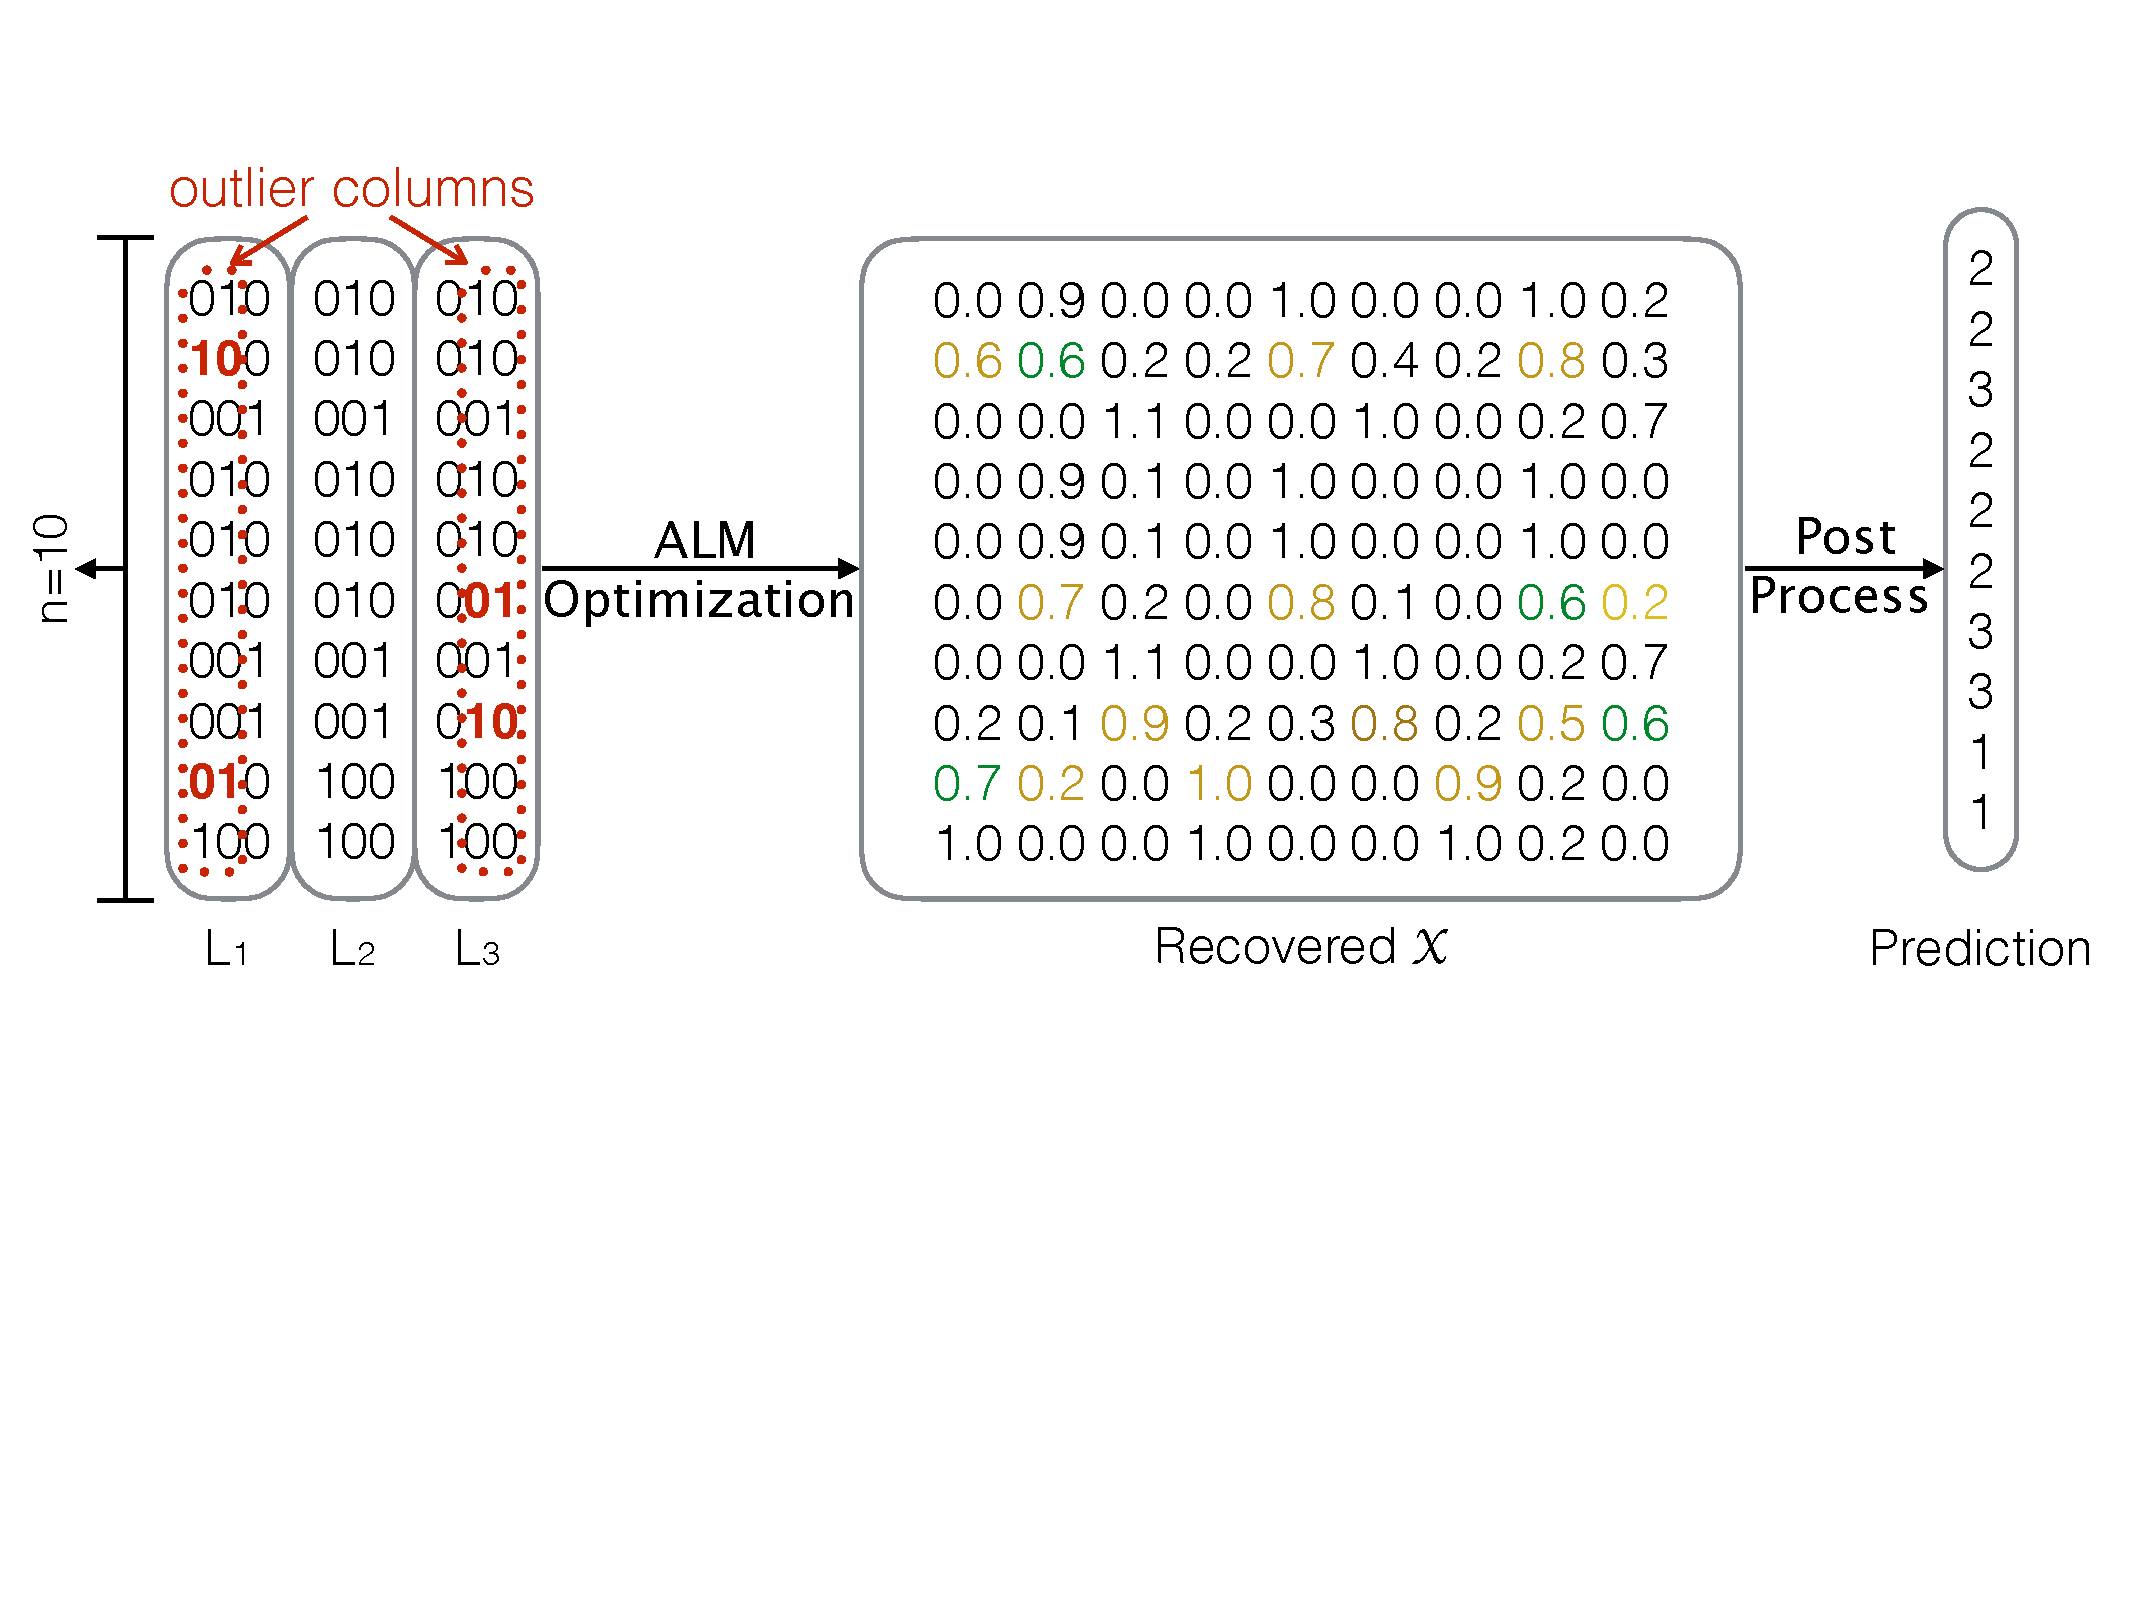
\includegraphics[width=0.46\textwidth]{resource/frame_work.pdf}
\end{center}
\caption{Framework of our late fusion algorithm.
In this example, there are 10 instances 3 classifiers and 3 classes.
Predictions of each classifier are converted to a binary indicator matrix,
denoted by $L_1$, $L_2$ and $L_3$.
Let $L = [L_1, L_2, L_3]$ be the label matrix.
Our algorithm detects and removes the outliers on $L$ and then recover the underlying low-rank subspace of $L$ as the prediction for testing instances.
We finally apply a post-processing method to generate the fused results.
%First, there are $\calC=3$ classifiers' results for $n=10$ instances.
%Each of them are converted into ``binary'' indicators from the soft prediction results, as $L = [L_1, L_2, L_3]$.
%Then, our ALM-based optimization process the binary indicator matrix into a recovered matrix $X$,
%which can be treated as soft prediction scores for testing instances.
%Finally, the fused prediction results are generated by a post-processing method.
}
\label{fig:framework}
\end{figure}

To avoid the expensive nuclear norm minimization,
in this paper, we propose a more efficient matrix factorization algorithm to recover the underlying low-rank label matrix.
Particularly, our method searches the solution in a low-rank subspace under a fixed-rank constraint.
This is a hard constraint, and it is different from~\cite{gaoijcai2016robust,ye2012robust} which introduce a soft constraint on the low-rank property.
On the other hand, to remove the abnormal predictions generated by individual features, we propose to filter out these inconsistent results by using the $\ell_{1,2}$ regularization (See Fig.\ref{fig:framework}.
Notations are introduced shortly.).
Specially, $\ell_{1,2}$ loss preserves the fidelity within each column by $\ell_{2}$ loss in the vertical direction and is robust to sparse errors across all the columns by $\ell_{1}$ loss in the horizontal direction.
Compared to $\ell_{1,2}$ loss, $\ell_{2}$ loss is sensitive to outliers, so that may not produce robust and satisfactory predictions.
$\ell_{1}$ loss is not sensitive to outliers, but not capable to detect the abnormal features which generate corrupted results.
In addition, most existing matrix factorization optimization methods only consider smooth loss functions, rather than the non-smooth loss.
Thus, we in particular present an approach based on augmented Lagrangian multiplier (ALM) to extend matrix factorization methods to non-smooth problems.

The main contributions are summarized as follows:
\begin{itemize}
  \item We formulate the late fusion problem as a fixed-rank robust matrix recovery problem, which is the first attempt to introduce a hard constraint on the low-rank property to the late fusion problem.
      Our model intuitively removes inconsistent predictions made by abnormal features and preserves the consistency of predictions from different sources.
  \item We propose an ALM-based algorithm to enable matrix recovery algorithms to handle non-smooth $\ell_{1,2}$ loss, rather than a simple least square loss which has been frequently studied in literature.
  %\item Our proposed algorithm is more efficient than most state-of-the-art late fusion methods.
  %It is capable of handling large scale problems.
  \item We provide theoretical convergence analysis for the proposed robust matrix recovery algorithm.
  \item Empirical studies show significantly improvement of our proposed method compared to existing late fusion andalgorithms and feature fusion methods.
\end{itemize}

\section{Related Work}
%% Matrix factorization
%% Fusion Methods

%MKL based method is a simple but efficient way to combine different features for multi-model fusion,
%and many improved algorithms have been proposed by introducing more constraint, boosting methods and other optimization.
MKL is a common way to combine different features for multi-model fusion.
In~\cite{vedaldi2009multiple}, the authors use MKL to learn an optimal combination of exponential ${\chi}^2$ kernels capturing a different feature channel.
Gehler \etal \cite{gehler2009feature} propose boosting approaches to ensemble different features, which learns the correct weighting of multiple predicted confidence scores from different models.
The authors of \cite{natarajan2012multimodal} propose a two-step strategy employing MKL and late score fusion methods to combine diverse features, specifically on event detection tasks.
In~\cite{lai2015learning}, a sample specific late fusion based on graph Laplacian with RankSVM style constraints is proposed,
which learns sample specific fusion weights by diffusing the information from labeled samples to the unlabeled one.
Xu \etal \cite{xuiccv2013feature} propose an optimization algorithm to combine diverse decision values,
which learns the weights, thresholding and smoothing parameters in a joint framework.
However, all these MKL based fusion methods or others only learn weights to combine different basic models, which do not consider the outlier rejection in the fusion process specifically.

%Our proposed late fusion algorithm is based on matrix factorization,
%which has attracted increasing attention recently.
Matrix factorization has attracted increasing attention recently.
Many manifold optimization algorithms on matrix factorization have been proposed by exploiting the manifold geometry in a subspace.
Based on manifold optimization, fixed-rank matrices are supposed to belong to a smooth matrix manifold~\cite{vandereycken2013lowrank,rtrmc2011boumal,Bonnabel2011,ngonips2012scaled}.
For instance, in~\cite{vandereycken2013lowrank}, the authors propose a low-rank geometric conjugate gradient (LRGeomCG) method.
In~\cite{rtrmc2011boumal}, first- and second-order Riemannian trust-region methods are applied to solve the low-rank matrix completion by exploiting the low-rank constraint.
In~\cite{Bonnabel2011}, a linear regression algorithm is proposed, where the parameter of this algorithm is a fixed-rank matrix based on the Riemannian manifold geometry.
%In~\cite{Mishra2012}, the authors propose a quotient geometric matrix completion method.
%The authors in~\cite{grouse2010Balzano} propose an online algorithm for tracking subspaces, Grassmannian rank-one update subspace estimation.
In~\cite{ngonips2012scaled}, a gradient methods based on scaled metric on the Grassmann manifold is proposed.
The authors in~\cite{Wen2012} propose a low-rank matrix fitting algorithm to solve large scale matrix completion problems by exploiting nonlinear successive over-relaxation.
In~\cite{RechtNIPS2011hogwild}, a lock-free approach to parallelizing stochastic gradient descent is proposed.
In \cite{jain2013low} the authors propose a alternating minimization method for matrix factorization with a global optimality guarantee,
but they require the incoherent matrix assumption and a fresh measurements at each iteration.
Thus their method cannot be guaranteed the global optimality in our work.
In addition, as shown in \cite{vandereycken2013lowrank}, the Riemannian manifold method may converge faster than the alternating minimization approach.
However, most existing matrix factorization methods only consider the general least square loss, which cannot be directly applied to handle $\ell_{1,2}$ loss.

Some other fusion algorithms are proposed for specific tasks.
The authors of \cite{zheng2015query} estimate a feature’s effectiveness in a query-adaptive manner for image retrieval problems,
and they combine the scores of multiple features weighted by their effectiveness.
Zha \etal \cite{zha2015exploiting} use fusion features scores of different CNN layers and encoded features improve the accuracy of action recognition.
In~\cite{feichtenhofer2016convolutional}, the authors explore a variety of fusion methods to combine spatial and temporal CNN models, significantly improving the performance of two-stream network~\cite{simonyan2014two}.
\cite{wangmodality} proposes a framework use high-dimensional Fisher Vector features from RGB, HHA and surface normal modalities to effectively achieve state-of-the-art scene classification performance.
\cite{Wang_Transformation,yaohighlight} use some simple strategies to choose specific weight for different scores from multiple features.
The authors in~\cite{vanicassp2014late} point out that missing values in predictions can be a challenge for late fusion due to the absence of features.
These special designed fusion algorithms can be hard to extend to general problems, being lack of generalization.



\section{The Proposed Approach}


We first elaborate the formulation of our proposed algorithm,
which regards the late fusion problem as a robust matrix recovery problem.
Then we present the details of using ALM extending matrix factorization to handle $\ell_{1,2}$ loss.
Finally we introduce our post-process strategy to convert the recovered label matrix to final predictions.

\subsection{Problem Formulation}

Suppose there are $n$ testing instances and $\calC$ classes.
We denote each instance as $x_i \in \dsR^{d}$ where $1 \leq i \leq n$.
Assume that we have already trained $m$ classifiers, \ie. $f_1, f_2, ... f_m$.
Then by applying each single classifier $f_j$ ($1 \leq j \leq m$) on the entire testing data, one can derive an indicator matrix $\bL_j \in \dsR^{n \times \calC}$, where $\bL_{j, ic} = 1$ if the $i$-th instance is assigned to the $c$ class, otherwise $\bL_{j, ic} = 0$ (as shown in Figure~\ref{fig:framework}).
Let $\bL = [ \bL_1, \bL_2, ..., \bL_m ]$.
%%On one hand, we aim to preserve the consistency among $m$ classifiers, so we introduce a rank-$m$ constraint on $\bL$.
On one hand, we aim to preserve the consistency among $m$ classifiers, so we introduce a rank constraint on $\bL$.
On the other hand, to catch the outlier columns, we apply robust $\ell_{1, 2}$ loss, which is computed by
{\small
\begin{align}
|| \bX ||_{1,2} = \sum_{j = 1}^{m\calC} \sqrt{ \sum_{i = 1}^{n} \bX_{ij}^2 }
\end{align}
}\noindent
Thus, a general formulation of recovering the underlying low-rank label matrix can be written as follows:
{\small
\begin{align}\label{eq:l12_rankconstraint}
  \min_{\bX} ~&~ || \calP_{\Omega} (\bL - \bX) ||_{1,2}~~~~~~\st~~\rank(\bX) = p
\end{align}
}
\noindent
where $\bX \in \dsR^{n \times m\calC}$ is the underlying low-rank label matrix to be recovered, $\rank(\bX)$ obtains the rank of $\bX$,
$\Omega$ denotes a subset containing the indices of the observed entries,
and $p$ is a scalar.
Here $\calP_{\Omega}$ denotes the orthogonal projection onto the linear space of matrices support on $\Omega: \calP_{\Omega}(\bX) = \bX_{ij}$ if $(ij) \in \Omega$; $\calP_{\Omega} = 0$ otherwise.
This includes some cases where missing elements may occur~\cite{vanicassp2014late}.
In our setting, to preserve the consistency among various classifiers, we set the hard constraint of the rank, \ie, $p = \calC$.



It is difficult to optimize Problem~(\ref{eq:l12_rankconstraint}) directly due to the presence of the rank constraint.
We hence transform the original problem as a matrix factorization formulation as follows:
{\small
\begin{align}\label{eq:l12_mf}
  \min_{\bX} || \calP_{\Omega}(\bL - \bX) ||_{1,2} ,~  \st~ \rank(\bX) = p  .
\end{align}
}
\noindent
Nevertheless, existing matrix factorization algorithms focus on smooth loss functions, rather than a non-smooth $\ell_{1,2}$ loss function~\cite{vandereycken2013lowrank,Wen2012,ngonips2012scaled,rtrmc2011boumal}.
In the following section, we present an ALM optimization framework to solve Problem~(\ref{eq:l12_mf}).


\begin{algorithm}[ht]

\begin{algorithmic}

\REQUIRE $\bL \in \dsR^{n \times m\calC}$, rank($\bX$) = $p$

\STATE Initialize $\rho > 1$, $t = 0$, $\blambda_{0} = 0$, $\bE_{0} = 0$, and $\mu_{0} > 0$.

\WHILE{$t = 0$ or $L_1(\bE_{t+1}-\bE_{t}) \geq \epsilon$}

  \WHILE{not converge}

    \STATE 1: Obtain $\bX_{t+1}$ by solving Problem~(\ref{eq:subproblem_wrt_X}).

    \STATE 2: Obtain $\bE_{t+1}$ by solving Problem~(\ref{eq:column_wise_soft_thresholding}).

  \ENDWHILE

  \STATE 3: $\blambda_{t+1} = \blambda_{t} + \mu_{t} (\calP_{\Omega}{(\bL - \bX_{t+1} - \bE_{t+1})})$.

  \STATE 4: $\mu_{t+1} = \rho \mu_{t}$.

  \STATE 5: t = t + 1.

\ENDWHILE

\ENSURE $\bX \in \dsR^{n \times m\calC}$

\end{algorithmic}
\caption{The ALM algorithm for Problem~(\ref{eq:mf_l21_constrained})}
\label{alg:alm_mf}
\end{algorithm}

\subsection{Optimization Based on ALM}

Most existing matrix factorization optimization methods only consider smooth loss functions, rather than the non-smooth $\ell_{1,2}$ loss used in Problem~(\ref{eq:l12_mf}).
In this section, we present an ALM based algorithm to optimize Problem~(\ref{eq:l12_mf}).


By introducing a new variable $\calP_{\Omega} (\bE) = \calP_{\Omega} (\bL - \bX)$, we can develop Problem~(\ref{eq:l12_mf}) as below:
{\small
\begin{align}\label{eq:mf_l21_constrained}
  \min_{\bE, \bX} ~&~ || \bE ||_{1,2}      \nonumber \\
  \st             ~&~ \calP_{\Omega} (\bE) = \calP_{\Omega} (\bL - \bX)  ,~ \rank(\bX) = p  .
\end{align}
}
\noindent
The augmented Lagrangian function of Problem~(\ref{eq:l12_mf}) is constructed as below
{\small
\begin{align}\label{eq:lagrangian_l21}
  \calL (\bX, \bE, \blambda, \mu) = &~ || \bE ||_{1,2} + \langle \blambda, \calP_{\Omega} (\bL - \bX - \bE) \rangle      \nonumber \\
                                    & + \frac{\mu}{2} || \calP_{\Omega} (\bL - \bX - \bE) ||_F^2
\end{align}
}
\noindent
where $\rank (\bX) = p$, $\mu$ is a scalar,
and $\blambda \in \dsR^{n \times m\calC}$ are the Lagrangian multipliers.
Here $\langle \bA, \bB \rangle$ is the inner product of $\bA \in \dsR^{m \times n}$ and $\bB \in \dsR^{m \times n}$, and defined as $\langle \bA, \bB \rangle = \sum_{i=1}^{n} \sum_{j=1}^{m} \bA_{ij} \bB_{ij}$.
Then we can update $\bX$ and $\bE$ alternatively, which is summarized in Algorithm~\ref{alg:alm_mf}.
The following lemma and theorem provide the theoretical convergence guarantee of the proposed algorithm.
We emphasize that our problem is a non-convex problem with a rank constraint, which is rarely studied in previous literatures.


\begin{lemma}
Given that the sequence $\{ \mu_{t} \}$ is always increasing, $\mu_{0} > 0$ and $\blambda_{0} = 0$, the sequence $\{ \blambda_{t} \}$ computed by Algorithm~\ref{alg:alm_mf} is bounded.
\end{lemma}

\begin{proof}
  The proof can be found in Appendix A.
  \mycomment{
  By the optimality of $\bE_{t+1}$ in Step 2 in Algorithm~\ref{alg:alm_mf}, we have the sub-differential of $\calL$ w.r.t. $\bE$ as zeros:
  {\small
  \begin{align}
  \label{eq:derivatives_calL_E}
    0 & \in \frac{\calL(\bX_{t+1}, \bE_{t}, \blambda_{t}, \mu_{t})}{\bE_{t+1}} \nonumber \\
      & = \partial(|| \bE_{t+1} ||_{1,2}) + \blambda_{t} + \mu_{t} (\calP_{\Omega} (\bL - \bX_{t+1} - \bE_{t+1})) \nonumber \\
      & = \partial(|| \bE_{t+1} ||_{1,2}) + \blambda_{t+1}   \nonumber \\
    \Rightarrow & -\blambda_{t+1} \in \partial(|| \bE_{t+1} ||_{1,2})  .
  \end{align}
  }
  \noindent
  Consider the computation of $\bE_{t+1}$ in Eq~(\ref{eq:column_wise_soft_thresholding}), which is associated with $\bL, \bX_{t+1}$, $\blambda_{t}$ and $\mu_{t}$.
  $\bL$ is the observation and thus bounded.
  $\bX_{t+1}$ is bounded due to the convergence guarantee of Step 1 in Algorithm~\ref{alg:alm_mf}~\cite{vandereycken2013lowrank}.
  $\{ \blambda_{t} \}$ is initialized by setting $\blambda_{0} = 0$ and $\{ \mu_{t} \}$ is non-decreasing.
  Thus when updating by Algorithm~\ref{alg:alm_mf}, $\bE_{t+1}$, $\partial(\bE_{t+1})$ and $\blambda_{t}$ are all bounded accordingly as $t$ increases.
  This completes the proof.
  }
\end{proof}

\begin{theorem}
\label{theorem:alm_convergence}
  Suppose the sequences $\{\bX_k\}_{k=1}^{\infty}$, $\{\bE_k\}_{k=1}^{\infty}$ and $\{\blambda_k\}_{k=1}^{\infty}$ are generated by Algorithm~\ref{alg:alm_mf}.
  As $k \to \infty$, the gradients of $\calL$ w.r.t. $\bX$ and $\bE$ vanish,
  thus any accumulation point $(\bX^*, \bE^*)$ is a stationary point.
\end{theorem}

%\vspace{1cm}
\begin{proof}
\label{proof:proof_AA}
  The proof can be found in Appendix B.
\end{proof}


\subsection{Subproblem Optimization w.r.t. $\bX$}
\label{sec:sub_x}

To update $\bX$, we have the following augmented Lagrangian function \wrt. $\bX$:
{\small
\begin{align}\label{eq:langrangian_wrt_X}
  \calL (\bX) = & \langle \blambda, \calP_{\Omega} (\bL - \bX - \bE) \rangle + \frac{\mu}{2} || \calP_{\Omega} (\bL - \bX - \bE) ||_F^2  \nonumber  \\
              = & \frac{\mu}{2} || \calP_{\Omega} (\bM - \bX) ||_F^2 - \frac{1}{2\mu}|| \blambda ||_F^2   ,
\end{align}
}
\noindent
where $\bM = \bL - \bE + \frac{\blambda}{\mu}$.
Hence, we derive the following subproblem \wrt. $\bX$:
{\small
\begin{align}\label{eq:subproblem_wrt_X}
  \min_{\bX} || \calP_{\Omega} (\bM - \bX) ||_F^2,~ \st~ \rank(\bX) = p.
\end{align}
}
\noindent
%Problem~(\ref{eq:subproblem_wrt_X}) contains a smooth loss function \wrt. $\bX$, thus can be efficiently solved by existing fixed-rank matrix factorization optimization algorithms, such as LRGeomCG~\cite{vandereycken2013lowrank}.
Problem~(\ref{eq:subproblem_wrt_X}) contains a smooth loss function of $\bX$.
We thus propose to solve the subproblem by exploiting Riemannian geometry of smooth fixed-rank matrices, which is briefly presented below.



The key idea of manifold optimization is that the update of $\bX$ is always performed on the same manifold, which ensures the rank of $\bX$ unchanged as the optimization iterates.
In other words, we search the solution for $\bX$ in a low-rank subspace.
A smooth manifold of fixed-rank-$\ranksym$ matrices is defined as~\cite{vandereycken2013lowrank}:
{\small
\begin{align}
\M_{\ranksym} &= \{\bX\in \R^{n\times m\calC}: \rank(\bX) = \ranksym\} \nonumber \\
       &= \{\U\diag(\bsigma)\V^{\trsp}: \U \in \textrm{St}_{\ranksym}^{n}, \V \in
           \textrm{St}_{\ranksym}^{m\calC}, ||\bsigma||_0 = \ranksym\} \nonumber
\end{align}
}
\noindent
where $\textrm{St}_{\ranksym}^{n} = \{\U \in \R^{n\times \ranksym}:
\U^{\trsp}\U = \I \}$ denotes the Stiefel manifold of $n \times \ranksym$ real and orthonormal matrices.
We denote the tangent space by $T_{\bX}\M_{\ranksym}$ of $\M_{\ranksym}$ at $\bX = \U\diag(\bsigma)\V^{\trsp} \in \R^{n \times m\calC}$,
which is obtained as below:
{\small
\begin{align}
\label{eq:tangent_vector}
&&T_{\bX}\M_{\ranksym} =  \{\U\bM\V^{\trsp} \!\!+\! \U_{\symp} \V^{\trsp} \!\!+\!
\U\V_{\symp}^{\trsp}: \bM \in \R^{\ranksym \times \ranksym}, \nonumber\\ && \U_{\symp} \in \R^{n\times \ranksym},
\U_{\symp}^{\trsp}\U = \0, \V_{\symp} \in \R^{m\calC \times \ranksym}, \V_{\symp}^{\trsp}\V = \0\}.
\end{align}
}
\noindent
One can define a metric $g_{\bX}({\bA},{\bB}) = \langle{\bA},{\bB}\rangle$ on $\M_{\ranksym}$,
with $\bX \in \M_{\ranksym}$ and ${\bA},{\bB} \in T_{\bX}\M_{\ranksym}$,
then $\M_{\ranksym}$ becomes a Riemannian manifold by restricting
$\langle\bA,\bB\rangle$
to the \emph{tangent bundle}, defined as the disjoint union of all tangent spaces:
$T\M_{\ranksym} = \bigcup_{\bX\in \M_{\ranksym}}\{\bX\} \times T_{\bX}\M_{\ranksym}
         = \! \{(\bX,\bP)\in \R^{n \times m\calC} \times \R^{n \times m\calC}: \bX \in \M_{\ranksym}, \bP \in T_{\bX}\M_{\ranksym}\}.$


Let $f(\bX) = ||\calP_{\Omega} (\bM - \bX) ||_F^2$.
%Suppose that $\G$ is the gradient of the smooth function $f(\bX)$ in Euclidean space at $\bX = \U\diag(\bsigma)\V^{\trsp} $.
Suppose that $\G = \nabla f(\bX)$ in Euclidean space at $\bX = \U\diag(\bsigma)\V^{\trsp}$.
Then, according to~\cite{vandereycken2013lowrank}, the Riemannian gradient of $f(\bX)$ on $\M_\ranksym$ is given as the orthogonal
projection of $\G$ onto the tangent space at $\bX$:
{\small
\begin{eqnarray}\label{eq:grad}
\grad{f(\bX)} = P_{T_{\bX}\M_{\ranksym}}(\G)
\end{eqnarray}
}
\noindent
where
$P_{T_{\bX}\M_{\ranksym}}(\bZ): \bZ \mapsto P_{U}\bZ P_{V} + P_{U}^{\perp} \bZ P_{V} + P_{U} \bZ P_{V}^{\perp}$
denotes the orthogonal projection of any
$\bZ \in \R^{n \times m\calC}$ onto the tangent space at $\bX = \U\diag(\bsigma)\V^{\trsp}$.
Here $P_U = \U \U^{\trsp}$ and $P_U^{\perp} = \I - \U \U^{\trsp}$ for any $\U \in \textrm{St}_{\ranksym}^{n}$.

\begin{lemma}
  Assuming that $\U_{\symp}$, $\V_{\symp}$ and $\bM$ are computed by Algorithm~\ref{alg:compute_riemannian_grad},
  we can obtain {${\textnormal{grad}} f(\bX) = \U \bM \V + \U_{\symp} \V^{\trsp} + \U \V^{\trsp}_{\symp}$}.
\end{lemma}

\begin{proof}
  The proof can be found in Appendix C.
  \mycomment{
\begin{align}
\label{eq:proof_lemma1}
       & \grad f(\bX) \\
       & = \U \bM \V^{\trsp} + \U_{\symp} \V^{\trsp} + \U \V_{\symp}^{\trsp}  \nonumber \\
       & = \U(\U^{\trsp} \G \V) \V^{\trsp} + (\bR_{v} - \U \bM) \V^{\trsp} + \U (\bR_{u} - \V \bM^{\trsp})^{\trsp} \nonumber \\
       & = P_{\U} \G P_{V} + \G \V \V^{\trsp} - \U \bM \V^{\trsp} + \U \U^{\trsp} \G - \U \bM \V^{\trsp} \nonumber \\
       & = P_{\U} \G P_{V} + \G P_{V} - 2\U \bM \V^{\trsp} + P_{U} \G  \nonumber \\
       & = P_{\U} \G P_{V} + \G P_{V} - 2\U (\U^{\trsp} \bR_{v}) \V^{\trsp} + P_{U} \G  \nonumber \\
       & = P_{\U} \G P_{V} + \G P_{V} - 2\U (\U^{\trsp} \G \V) \V^{\trsp} + P_{U} \G  \nonumber \\
       & = P_{\U} \G P_{V} + (\bI - P_{U}) \G P_{V} + P_{U} \G (\bI - P_{V})  \nonumber \\
       & = P_{\U} \G P_{V} + P_{U}^{\perp} \G P_{V} + P_{U} \G P_{V}^{\perp}  ,
\end{align}
}
\end{proof}


\begin{algorithm}
  \begin{algorithmic}
    \REQUIRE $\bX = \U \diag(\sigma) \V^{\trsp} \in \M_{r}$, $\G$.
    \STATE 1. $\bR_{u} \leftarrow \G^{\trsp} \U$, $\bR_{v} \leftarrow \G \V$.
    \STATE 2. $\bM \leftarrow \U^{\trsp} \bR_{v}$.
    \STATE 3. $\U_{\symp} \leftarrow \bR_{v} - \U \bM$, $\V_{\symp} \leftarrow \bR_{u} - \V \bM^{\trsp}$.
    \ENSURE $\grad f(\bX) = \U \bM \V^{\trsp} + \U_{\symp} \V^{\trsp} + \U \V_{\symp}^{\trsp} \in T_{\bX}\M_{\ranksym}$.
  \end{algorithmic}
  \caption{Computation of $\grad f(\bX)$ (Algorithm 2 in~\cite{vandereycken2013lowrank})}
  \label{alg:compute_riemannian_grad}
\end{algorithm}


\begin{algorithm}
  \begin{algorithmic}
    \REQUIRE Initial $\bX_{1} \in \M_{\ranksym}$, tangent vector $\bfeta_{0} = \0$, $k = 1$.

    \WHILE{not converge}

      \STATE 1. Compute Riemannian gradient $\bP_{k} = \grad f(\bX_{k})$ by Algorithm~\ref{alg:compute_riemannian_grad}.

      \STATE 2. Compute a conjugate direction with PR+:
             $\bfeta_k = - \bP_{k} + \beta_{k} \mT_{\bX_{k-1} \rightarrow \bX_{k}}( \bfeta_{k-1}) \in T\M_{\ranksym}$.

      \STATE 3. Find a step size $t_{k} = \min_{t} f(\bX + t\bfeta_{k}) $

      \STATE 4. Update $\bX_{k+1} = R_{\bX_{k}}(t_{k} \bfeta_{k})$.

      \STATE 5. $k = k + 1$.

    \ENDWHILE

    \ENSURE $\bX \in \M_{\ranksym}$.

  \end{algorithmic}
  \caption{LRGeomCG (Algorithm 1 in~\cite{vandereycken2013lowrank})}
  \label{alg:LRGeomCG}
\end{algorithm}


Based on the above discussion, the solution of $\bX$ can be solved by Algorithm~\ref{alg:LRGeomCG}.
Particularly, in Step 2 of Algorithm~\ref{alg:LRGeomCG}, $\beta_{k}$ is determined by a Polak-Ribi$\grave{e}$re (PR+) rule~\cite{vandereycken2013lowrank}:
{\small
\begin{eqnarray}\label{eq:beta}
\beta_{k} = \frac{\grad f(\bX_{k})^{\trsp}(\grad f(\bX_{k}) - \grad f(\bX_{k-1}))}{\langle \grad f(\bX_{k-1}),\grad f(\bX_{k-1})\rangle}.
\end{eqnarray}
}
\noindent
The step size $t_{k}$ in Step 3, given a search direction $\bfeta_{k} \in T_{\bX_{k} \M_{\ranksym}}$, is chosen such that
{\small
\begin{align}\label{eq:choose_step_size}
  f(R_{\bX_{k}} (t_{k} \bfeta_{k})) \leq f(\bX_{k}) + c_{1} t_{k} \langle \grad f(\bX_{k}), \bfeta_{k} \rangle ,
\end{align}
}
%\begin{align}\label{eq+choose_step_size2}
%  | \langle \grad f(R_{\bX_{k}} (t_{k} \bfeta_{k})), & \mT_{\bX_{k-1} \rightarrow \bX_{k}} (\bfeta_{k}) \rangle |  \nonumber \\
%                           & \leq c_{2} | \langle \grad f(\bX_{k}), \bfeta_{k} \rangle |  ,
%\end{align}
\noindent
where $0 \leq c_{1} \leq c_{2} \leq \frac{1}{2}$.
The notation $\mT_{\bX_{k-1} \rightarrow \bX_{k}} (\bfeta_{k-1})$ in Step 2 and $R_{\bX_{k}} (t_k \bfeta_{k})$ denote \emph{vector transport} and \emph{retraction}, respectively.
For more details of above two operators and the geometry of $\M_{\ranksym}$, see~\cite{vandereycken2013lowrank} and the references therein.



\subsection{Subproblem Optimization w.r.t. $\bE$}

Similarly, to update $\bE$, we have the following problem \wrt. $\bE$:
{
\begin{align}
\label{eq:subproblem_wrt_E_2}
  \min_{\bE} & || \bE ||_{1,2} + || \calP_{\Omega} (\bN - \bE) ||_F^2 ,
\end{align}
}
\noindent
where $\bN = \bL - \bX + \frac{\blambda}{\mu}$.
The above problem can be efficiently solved by the following column-wise soft-thresholding operator~\cite{xiao2015FaLRR}:
{
\begin{align}\label{eq:column_wise_soft_thresholding}
  \bE_{i} = \calS_{\alpha}(\bN_{i}) = \left\{
    \begin{aligned}
      & \zerocolumn,~\text{if}~ ||\calP_{\Omega} (\bN_{i})||_2 \leq \alpha   \\
      & \calP_{\Omega} (\bN_{i}) - \frac{\alpha \calP_{\Omega} (\bN_{i})}{|| \calP_{\Omega} (\bN_{i}) ||_2},~\text{otherwise,}
    \end{aligned}
    \right.
\end{align}
}
\noindent
where $\bE_{i}$ and $\bN_{i}$ denote the $i$-th column of $\bE$ and $\bN$,
and $\alpha = \frac{1}{2}$.

\subsection{Post Process}
As we recover the low-rank matrix $\bX$ from the label assignment matrix $\bL$,
there requires a post process to generate the prediction label for each testing data from $\bX$.
Intuitively, there might be several possible methods to select as below:

\begin{itemize}
  \item \textbf{[AVE].} A prediction score matrix $\bX^{*} \in \dsR^{n \times {\calC}}$ is obtained by averaging $[ \bX_1, \bX_2, ..., \bX_{\calC}]$.
    The indicator of the highest value in each row of $\bX^{*}$ is regard as the predicted label for the corresponding data.
  \item \textbf{[VOTE].} For $\bX_j$ where $1 \leq j \leq m$, we set $\bI_{ij}$ as the index of the highest value in the $i$-th row of $\bX_j$.
      Each $\bI_{ij}$ contributes one point to the $i$-th data with label $\bI_{ij}$.
      The label with the most votes is the final prediction result.
  \item \textbf{[GATE].} $\bX_j$ where $1 \leq j \leq m$ are transformed through softmax function as a gate of the corresponding confidence score matrix, which is normalized by $L_2$ norm.
      As $\bX_j$ contains outlier rejection information, we product the $\bX_j$ by the corresponding score matrix after softmax and normalization.
      The similar process as the first strategy is applied to predict the final labels.
\end{itemize}
According to the experiments, the last strategy ``GATE'' outperforms than the others.
So We choose the last one as the post process for our fusion method and analyze inner reasons during the experiment section.

\subsection{Computation Complexity}

%Now we analyze the computation complexity of our proposed algorithm.
%The sub-algorithm in Section~\ref{sec:sub_x} solve the solution of $\bX$.
For the optimization on $\bX$, the primary computation is described in Algorithms.~\ref{alg:compute_riemannian_grad} and~\ref{alg:LRGeomCG},
which uses subspace search to optimize the solution.
And the complexity is $T \times O((n+{\calC}m){\calC}^2)$, where $T$ is the number of iterations.
According to \cite{vandereycken2013lowrank}, $T$ is less than 100 for most situations,
and more details can be found in \cite{vandereycken2013lowrank}.
The complexity of optimization on $\bE$ and post-processing can be easily calculated as $O(nm{\calC})$ and $O(nm{\calC})$.
So, the total complexity per iteration is $T \times O((n+{\calC}m){\calC}^2) + O(nm{\calC})$,
which is linear by growing of $n$ and $m$, with the cubic complexity of $\calC$.

Comparing with those nuclear norm based methods~\cite{gaoijcai2016robust,ye2012robust} whose computational complexity is cubic due to the presence of SVDs,
our algorithm is more efficient for large scale problems.
For example, \cite{gaoijcai2016robust} reportes their entire complexity is $(m{\calC})^3+n(m{\calC})^2$ per iteration.
With the increase in the number of classifiers,
the computation costs too much to be affordable due to the cubic complexity of $m$,
but ours can still solve the solution.

\section{Experimental Studies}

\begin{table*}[t]
\centering
\begin{tabular}{|c|c|c|c|c|c|}
\hline
Method         & UCF-101          & CIFAR-10         & CIFAR-100        & Oxford-IIIT-Pet  & PASCAL VOC 2007    \\\hline
ASF            & 86.78\%          & 94.21\%          & 76.91\%          & 92.46\%          &   90.51\%          \\
MKL            & 85.38\%          & 94.15\%          & 72.71\%          & 87.13\%          &   85.82\%          \\
RCEC           & 86.60\%          & 94.99\%          & 77.13\%          & 92.11\%          &   90.92\%          \\
FWOT           & -                & -                & -                & \textbf{92.90\%} &   91.20\%          \\
LPBoost        & 86.24\%          & 94.88\%          & 76.59\%          & 92.73\%          &   \textbf{91.42\%} \\\hline
\textbf{Ours}  & \textbf{89.03\%} & \textbf{95.11\%} & \textbf{77.72\%} & \textbf{92.90\%} &   90.98\%          \\
\hline
\end{tabular}
\caption{Mean accuracy on real-world data sets.
FWOT costs excessive time for training UCF-101, CIFAR-10 , CIFAR-100~(over 24 hours),
so we omit these results indicated by ``-''.
}
\label{table:total_acc}
\end{table*}


\begin{table*}[t]
\centering
\begin{tabular}{|c|c|c|c|c|c|}
\hline
Method        & UCF-101         & CIFAR-10        & CIFAR-100        & Oxford-IIIT-Pet & PASCAL VOC 2007 \\\hline
RCEC          & \textbf{86.60}  & 81.41           &  \textbf{255.51} & \textbf{18.82}  &   16.45         \\
FWOT          & $\infty$        & $\infty$        &  $\infty$        & 61697           &   19674         \\
LPBoost       & 110.81          & 72.45           &  4750.9          & 43.67           &   \textbf{7.46} \\\hline
\bf{Ours}     & 421.23          & \textbf{5.384}  &  417.26          & 76.16           &   15.21         \\
\hline
\end{tabular}
\caption{Computational time on real-world data sets. Computational time is recorded in seconds.
FWOT costs excessive time for training UCF-101, CIFAR-10 , CIFAR-100~(over 24 hours),
so we omit these results indicated by ``$\infty$''.}
\label{table:total_time}
\end{table*}


\subsection{Synthetic Experiments}

We set $n = 280$, $m = 15$, $\calC = 20$ to generate $n$ instances, which are randomly labeled with $c_i, 1 \leq i \leq n, 1 \leq c_i \leq \calC$.
We regard these instances as the ground truth data represented by a matrix $Gt \in \dsR^{280 \times 1}$.
Then we randomly permute $40\%$ instances' labels,
repeating $m = 15$ times to get fifteen classifiers' results as $Er \in \dsR^{280 \times 15}$.
Therefore, the classification error of each classifier is around 40\%.
Then, we derive an indicator matrix from the predictions of 15 classifiers,
and recovery this indicator matrix into the final results, $Rec \in \dsR^{280 \times 15}$, by our proposed algorithm.
%Deriving an indicator matrix $\bL \in \dsR^{280 \times 300}$ from the synthetic classifiers' results as the input of our proposed algorithm,
%the visualization results are illustrated in Fig.~\ref{fig:ensemble_cluster}.
We visualize the ground truth information, classifiers' predictions and the recovered results in Fig.~\ref{fig:ensemble_cluster}.

\begin{figure}[ht]
\center
\subfigure[Ground Truth]{
\label{subfig:gt_pdf}
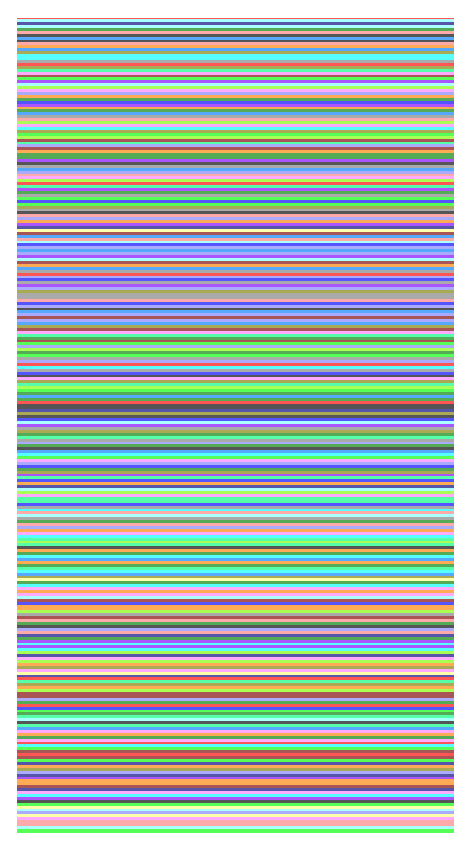
\includegraphics[width=0.14\textwidth]{resource/ground_truth.eps}
}
\subfigure[Random Noise]{
\label{subfig:er_pdf}
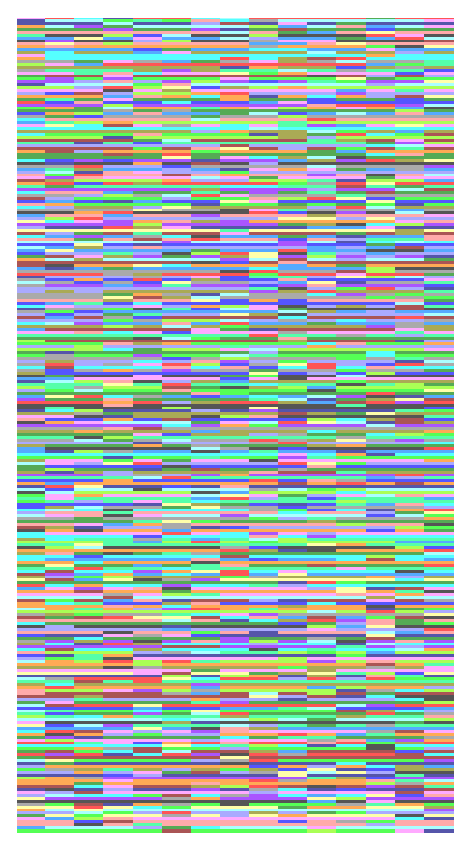
\includegraphics[width=0.14\textwidth]{resource/random_error.eps}
}
\subfigure[\bf{Our Results}]{
\label{subfig:re_pdf}
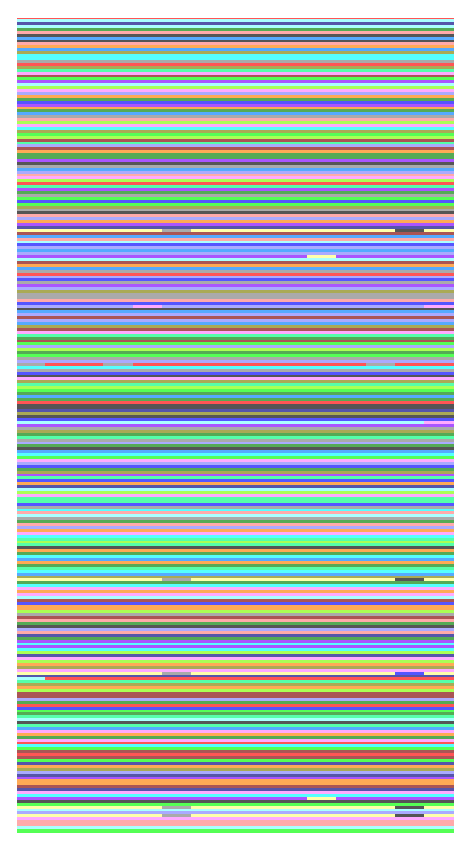
\includegraphics[width=0.14\textwidth]{resource/recover.eps}
}
\caption{Visualized results of the synthetic dataset.
Different colors represent different labels for each instance. 
Fig.~\ref{subfig:gt_pdf} show the visualized ground truth data, and each row corresponds to one instance with the class label represented by color.
Fig.~\ref{subfig:er_pdf} has 15 columns, each represents one classifiers's predictions.
There are also 15 columns in Fig.~\ref{subfig:re_pdf}, which is generated by the recovered results from our algorithm.
Obviously, most of the outlier elements are correctly recovered with only a few error predictions left.
}
\label{fig:ensemble_cluster}
\end{figure}

As we can observe, our proposed algorithm significantly detect the outliers.
Furthermore, the outlier elements are accurately converted into the correct predictions, and only few results are wrong.
This preserves the consistency among all classifiers.


\subsection{Real-world Experiments}

We evaluate the performance on eight publicly available real-world data sets,
UCF101~\cite{UCF101}, CIFAR-10~\cite{krizhevsky2009learning}, CIFAR-100~\cite{krizhevsky2009learning}, Oxford-IIIT-Pet~\cite{parkhi2012cats}, PASCAL VOC 2007~\cite{pascal-voc-2007}, Oxford Flower 17~\cite{nilsback2006visual}, Pascal Sentence~\cite{rashtchian2010collecting} and Wikipedia~\cite{rasiwasia2010new}.

\subsubsection{Feature Extraction}

We used the best-performing CNN models for feature extraction including GoogleNet~\cite{szegedy2015going}, ResNet~\cite{he2015deep}, ResNeXt~\cite{xie2016aggregated}, Pre-ResNet~\cite{he2016identity} and VGG~\cite{chatfield2014return} or etc.
These features are fairly state of the art.
They have been widely used in various recent research papers and have been verified the most effective features by recent internationally recognized competitions such as the ImageNet competition~\cite{russakovsky2015imagenet}.

On UCF101 dataset, five different features are extracted from the following:
`fc6' of C3D~\cite{tran2015learning}, `pool5/7x7\_s1' from GoogleNet, `pool5' of ResNet-152, and two `fc6's of Two-Stream~\cite{simonyan2014two}.
Given a video, we extract the above five features following the same process described in Two-Stream.

On Cifar10 dataset, the features are extracted from the global pooling layer of ResNet-20,32,44,56,110 and of Pre-ResNet-20,32,44,56,110,164 models.
One feature is extracted from the last pooling layer of cifar10\_full model described in caffe example prototxt.
Two modified networks VGG16 and GoogleNet are used to extract final pooling features~(Modify the stride 2 in conv4 and conv5 layers to stride 1 and fc layers to global pooling layers).
On Cifar100 dataset, we use `global\_pool' layer features of ResNet-20,32,44,56,68,110 and of Pre-ResNet-20,32,44,56,110,164 models.

In all other datasets, eight different features are extracted from the following: ``fc6'' of VGG16, VGG19, 
``fc6'' of AlexNet,CaffeNet~\cite{krizhevsky2012imagenet},
``pool5/7x7\_s1'' from GoogleNet, and ``pool5'' of ResNet-50,101,152.

\subsubsection{Late Fusion}
Five state-of-the-art late fusion methods are compared with our proposed algorithm.
Average Score Fusion (ASF): we directly average the results from multiple classifiers, then the $L_2$ norm is applied on each classifier's results for normalization.
Multiple Kernel Learning (MKL): MKL learns a weight coefficient $w$ for each classifier, and the final scores are obtained from function $f(s)=w^{T}s,~\sum w = 1$.
Robust Convex Ensemble Clustering (RCEC)\cite{gaoijcai2016robust}: we modify the core alogrithm in RCEC to recover $\bX$ from $L$ in Eq.~\ref{eq:l12_mf}, and use the same post process.
Feature Weighting via Optimal Thresholding (FWOT) \cite{xuiccv2013feature}: they propose to learn thresholding, smoothing parameters and weights in a joint framework to combine multiple prediction results.
LPBoost~\cite{gehler2009feature}: A variant linear combination is applied to multiple classifiers to boost performance.

The parameter $\mu$ is selected from $\{0.1, 1, 5\}$,
$\rho$ is select from $\{1.01, 1.05, 1.1\}$
and $\epsilon$ is select from $\{1e-2, 1e-3, 1e-4\}$ in all our experiments.
Among different parameters, there are only small differences of the prediction performance.
LIBLINEAR~\cite{fan2008liblinear} is adopted for our basic classification toolbox.
The parameters are set as default in LIBLINEAR and liblinear-mkl, unless otherwise specified.
For RCEC method, we use 5 folder cross validation to select the best parameter $\beta$ from $\{0.01,1,2,4,6,...,20\}$ and set $\lambda = 0.1, \gamma = 0.01$, which are suggested by author~\cite{yiicdm2012robust}.
For FWOT, the smoothing parameter candidates are $\{0.5, 0.6, ... , 0.9\}$ and the parameter $C$ in is selected from $\{10^{-4},10^{-2},...,10^{4}\}$ according to cross-validation, which is same in~\cite{xuiccv2013feature}.
For LPBoost, we use cross-validation to pick up the best $\nu$ from $\{0.5,0.6,0.7,0.8,0.9\}$ suggested in~\cite{xuiccv2013feature}.


Five datasets are used for late fusion comparison.
UCF 101 is commonly used for action recognition task, which has 9573 training videos and 3783 testing videos, categorized into 101 human action classes.
CIFAR-10 dataset contains 60000 pictures with 10 classes.
CIFAR-100 similar with CIFAR-10, except it, has 100 classes containing 600 images each.
The Oxford-IIIT-Pet dataset contains 7349 images covering 37 different breeds of cats and dogs.
PASCAL VOC 2007 is a dataset for general object detection and image classification.
We only use the image with a single class, which includes 6146 images.
For UCF 101, we use the official split-1 set for training and testing.
For Oxford-IIIT-Pet and PASCAL VOC 2007, we randomly sample fifty percent pictures as our training data and the others as testing data.
We repeat the sample, training and fusion process five times to get fair results.

Table~\ref{table:total_acc} shows the mean accuracy results for the five datasets, and our proposed algorithm provides a significant improvement compared with other effective late fusion methods on most datasets.
Additionally, our algorithm is more efficient than other late fusion methods in most situations.
As we can see from Table~\ref{table:total_time}, some methods are not capable of handling large scale datasets.
For example, FWOT is too slow to train; thus we do not show its result for UCF101 and CIFAR (more than one day).
The time consumption of ours is acceptable in all experiments and quite fast on CIFAR-10/VOC2007.
Our method and RCEC have the similar range of running time. Nevertheless, our method outperforms RCEC regarding accuracy for all the five datasets.
In conclusion, our method can handle the large scale problem efficiently and yield stable performance.

\subsubsection{Feature Fusion}
Feature fusion usually has some limitation when we combine too many models. For example, directly training a fusion model that fuses several CNN models may be intractable due to excessive GPU memory consumption.
We compare three different feature fusion methods in Table~\ref{table:feature}.
The Bayesian-based method \cite{chen2012bayesian} requires the same dimensionality of features for fusion.
Thus we choose the global-pooling layer's feature of all residual-based networks used in Table~\ref{table:total_acc} for \cite{chen2012bayesian}.
For the other two feature fusion methods, we directly concatenate the global-pooling layer (or the probability prediction layer) of the same networks in the Bayesian-based method; and use a fully connected layer with ten output to combine the concatenation feature to the final prediction for the CIFAR-10 dataset.
For our fusion algorithm, we use the CNN predictions rather than the SVM predictions used in Table~\ref{table:total_acc}.

\begin{table}[t]
\centering
\begin{tabular}{|c|c|c|c|}
\hline
   Bayesian  & Pooling Layer & Prob Layer   & \bf{Ours}     \\\hline
    94.10\%  & 95.21\%       &   95.32\%    & \bf{95.93\%}  \\
\hline
\end{tabular}
\caption{Mean accuracy on CIFAR-10 to compare different feature fusion methods with ours. Bayesian represents \cite{chen2012bayesian}, ``Pooling Layer''/``Prob Layer'' represent we concatenate the features from the last pooling layer/the probability layer.}
\label{table:feature}
\end{table}

From the Table~\ref{table:feature}, our method still achieves the best performance among these feature fusion methods.
Some other detailed comparison can be found Appendix D.


\subsection{Post Strategy Selection}

In this section, we compare three proposed post strategies on three datasets.
Wikipedia dataset \cite{rasiwasia2010new} contains paragraphs of text for each picture, and total 2866 image-text pairs are categorized into 10 class.
Oxford Flowers 17 \cite{nilsback2006visual} has seventeen flower categories with 80 images for each category.
Pascal Sentence \cite{Li2006One} contains 1000 images annotated by caption information and categorized into twenty classes.
Fifty percent of data are sampled as training set and the others as testing set, and experiments are repeated five times on above three datasets.

The $[$AVE$]$ strategy outperforms than the $[$VOTE$]$ in our experiments, which may be caused by the soft average method reserves more detail information than the hard voting method.
In all our experiments, the accuracy performance of the $[$GATE$]$ strategy is higher than the others.
Since the recover matrix $\bX$ contains the outlier rejection information,
it is more robust to take advantage of the recovered results as a confidence gate operating on the original confidence score matrix.

\begin{table}[ht]
\centering
\begin{tabular}{|c|c|c|c|}
\hline
Strategy            & Wikipedia         & Flowers 17          & Pascal Sentence     \\\hline
[AVE]               & 47.78\%           & \textbf{96.77\%}    & 66.40\%             \\\hline
[VOTE]              & 47.85\%           & 96.61\%             & 66.20\%             \\\hline
[GATE]              & \textbf{49.03\%}  & \textbf{96.77\%}    & \textbf{67.20\%}    \\
\hline
\end{tabular}
\caption{Mean accuracy using different post process strategies on three datasets.}
\label{table:strategy}
\end{table}

\subsection{Comparison with State-of-the-art Models}

We compare the performance of our algorithm with the state-of-the-art single models.
In the previous experiments, we use SVM classifiers based on different features to make a fair comparison with some MKL based methods.
The performance of SVM classifiers is usually not as good as the results directly predicted by CNN models.
In order to obtain a higher result, we directly use multiple state-of-the-art CNN predictions and fuse them by our method.
The models used for ``Ours$^{*}$'' in Table \ref{table:state_of_the_art} are shown in Table \ref{table:models}.
We demonstrate the improvement of our fusion results compared to the state-of-the-art single model performance in Table~\ref{table:state_of_the_art}.

\begin{table}[ht]
\centering
\begin{tabular}{| c | c | c |} \hline
                                           & CIFAR-10             & CIFAR-100  \\\hline
\multirow{2}{*}{ResNet} & 110, 134, 164    & 56, 110, 164  \\
                                           & $164^{*}$, $200^{*}$ & $110^{*}$, $164^{*}$  \\\hline
\multirow{2}{*}{WRN} & 16-10, 22-8, 28-10  & 16-10, 22-8, 28-10  \\
                                           &    40-4, 40-8        & 40-4  \\\hline
NIN                                        &     -                & -  \\ \hline
\end{tabular}
\caption{Model selection for CIFAR-10 dataset.
In the ResNet block, numbers represent the depth of the selected models.
``*'' represents using the bottleneck block, otherwise using the basic block in residual networks.
In WRN~\cite{zagoruyko2016wide} block, ``x-y'', x represents the depth, and y represents the widening factor.
NIN~\cite{lin2013network} has only one formula, so we do not list its depth.}
\label{table:models}
\end{table}

\begin{table}[ht]
\centering
\begin{tabular}{|c|c|c|}\hline
    Methods              &  CIFAR-10       & CIFAR-100           \\\hline
Highway                  &   7.72          &  32.39              \\\hline
Pre-ResNet (1001 layers) &   4.92          &  22.71              \\\hline
WRN-28-10                &   4.17          &  20.50              \\\hline
ResNeXt-29-16x16d        &   3.58          &  17.31              \\\hline
Ours$^{*}$               &   3.47          &  17.24              \\\hline
Ours (fuse ResNeXt)      &   \textbf{3.19} &  \textbf{16.99}     \\\hline
\end{tabular}
\caption{Test error of different methods on CIFAR-10 and CIFAR-100 for different architectures.
}
\label{table:state_of_the_art}
\end{table}

We carefully cite the best performances reported in their papers, Highway \cite{srivastava2015highway}, Pre-ResNet \cite{he2016identity}, WRN-28-10 \cite{zagoruyko2016wide}, ResNeXt-29-16x16d \cite{xie2016aggregated}.
As can be observed, our fusion algorithm is capable of further improving the performance of single models significantly,
even a single model has the satisfactory performance with deeper depth or wider channel.
We emphasize that ResNeXt is the best performer in single models, and our method only fuses models which perform worse than ResNeXt, but can achieve lower test error than ResNeXt.
Including the results of ResNeXt-29-16x16d in our fusion method, we can obtain a much lower test error.
This demonstrates the aim and benefit of our late fusion method.


\section{Conclusion}

Late fusion is proposed to improve prediction performance by taking advantages of multiple features together.
%In practice, the ubiquitousness of controversy of different features may degenerate the performance.
In practice, the controversy of different features is ubiquitous and may degenerate the performance.
To deal with this issue, we formulate this task as a robust matrix recovery problem with a hard constraint on the matrix rank to preserve the consistency among various features.
Matrix factorization is often considered to handle the hard rank constraint, but only focuses on smooth loss, while it is unclear how to extend them to handle non-smooth robust loss, \eg, $\ell_{1,2}$ loss.
We thus propose an ALM-based algorithm to cope with the non-smooth loss.
Empirical studies on large scale real-world data sets demonstrate that our proposed method can effectively improve performance compared to the state-of-the-art fusion methods.


{
\footnotesize
\bibliographystyle{aaai}
\bibliography{egbib}
}

\end{document}
